\chapter{Лабораторная работа №1. Статические методы оптимизации}

\section*{Постановка задачи}
Требуется найти минимум критерия качества для статической задачи оптимизации
\[
J(x,u)=5x^2+2u^2+3xu+4x+u-5,
\]
а также выполнить поиск экстремума градиентными методами. Вариант: \textbf{13}. Для пунктов с ограничениями используется функция ограничения
\[
 c(x,u)=4x^2+u+1.
\]

\section{Поиск глобального минимума на основе необходимых и достаточных условий}
\subsection{Случай без ограничений}
Найдём стационарную точку, приравняв к нулю градиент функции \(J(x,u)\):
\[
\nabla J(x,u)=\begin{bmatrix}\dfrac{\partial J}{\partial x}\\[2mm]\dfrac{\partial J}{\partial u}\end{bmatrix}
=\begin{bmatrix}10x+3u+4\\ 3x+4u+1\end{bmatrix}=\mathbf{0}.
\]
Получаем систему линейных уравнений
\[
\begin{cases}
10x+3u+4=0,\\
3x+4u+1=0.
\end{cases}
\]
Решая её, из второго уравнения выразим \(x=\dfrac{-1-4u}{3}\) и подставим в первое:
\[
\frac{-10-40u}{3}+3u+4=0 \;\Rightarrow\; -10-40u+9u+12=0 \;\Rightarrow\; 2-31u=0,
\]
откуда
\[
 u^{\ast}=\frac{2}{31},\qquad x^{\ast}=-\frac{13}{31}.
\]
Проверим достаточное условие минимума по положительной определённости матрицы Гессе:
\[
H=\begin{bmatrix}10&3\\3&4\end{bmatrix},\qquad \Delta_1=10>0,\quad \det H=10\cdot4-3^2=31>0.
\]
Следовательно, \(H\) положительно определена, а найденная стационарная точка является \textbf{единственным глобальным минимумом} квадратичной функции \(J\).

Значение критерия в точке минимума:
\[
J(x^{\ast},u^{\ast})=5\Big(\frac{13}{31}\Big)^2+2\Big(\frac{2}{31}\Big)^2+3\Big(-\frac{13}{31}\cdot\frac{2}{31}\Big)+4\Big(-\frac{13}{31}\Big)+\frac{2}{31}-5
= -\,\frac{5580}{961}\approx -5.804.
\]

% Далее будут пункты 1.2, 1.3 и раздел 2 (градиентные методы)

% --- Продолжение раздела 1: ограничения ---
\subsection{С ограничением вида равенства \(c(x,u)=0\)}
Пусть ограничение имеет вид \(c(x,u)=4x^2+u+1=0\). Используем метод Лагранжа для минизации \(J(x,u)\) при \(c(x,u)=0\). Рассмотрим функцию Лагранжа
\[
\mathcal{L}(x,u,\lambda)=J(x,u)+\lambda\,c(x,u)=5x^2+2u^2+3xu+4x+u-5+\lambda\,(4x^2+u+1).
\]
Необходимые условия первого порядка:
\[
\frac{\partial \mathcal{L}}{\partial x}=10x+3u+4+8\lambda x=0,\qquad
\frac{\partial \mathcal{L}}{\partial u}=4u+3x+1+\lambda=0,\qquad
c(x,u)=0.
\]
Исключая \(u\) из ограничения, имеем \(u=-1-4x^2\). Подстановка в условия даёт кубическое уравнение для \(x\):
\[
128x^3-36x^2+34x+1=0.
\]
Его действительный корень (единственный с учётом строгой выпуклости \(J\)) равен
\[
 x^{\ast}_{=}\approx -0.02847,\qquad u^{\ast}_{=}= -1-4(x^{\ast}_{=})^2\approx -1.00324.
\]
Поскольку матрица Гессе \(H\succ0\), \(J\) строго выпукла, то найденная стационарная точка на гладком многообразии \(c=0\) является единственным глобальным минимумом на множестве \(\{c=0\}\). Значение функционала
\[\small
J(x^{\ast}_{=},u^{\ast}_{=})\approx -4.014.
\]
Для численной проверки и воспроизводимости ниже приведён короткий скрипт, который решает условия ККТ и вычисляет значения:

\begin{lstlisting}[caption={Решение условий ККТ для равенства и проверка},label={lst:kkt}]
# lab1/python/task1_kkt.py
import sympy as sp
x,u,lam = sp.symbols('x u lam', real=True)
J = 5*x**2 + 2*u**2 + 3*x*u + 4*x + u - 5
c = 4*x**2 + u + 1
L = J + lam*c
sol = sp.nsolve([
    sp.diff(L,x),
    sp.diff(L,u),
    c
],[x,u,lam], (-0.03, -1.0, 3.0))
print({"x": float(sol[0]), "u": float(sol[1]), "lambda": float(sol[2]), "J": float(J.subs({x:sol[0],u:sol[1]}))})
\end{lstlisting}

\subsection{С ограничением вида неравенства \(c(x,u)\le 0\)}
Сначала проверим допустимость найденного безусловного минимума \((x^{\ast},u^{\ast})=\big(-\tfrac{13}{31},\tfrac{2}{31}\big)\):
\[
 c(x^{\ast},u^{\ast})=4(x^{\ast})^2+u^{\ast}+1=4\Big(\tfrac{13}{31}\Big)^2+\tfrac{2}{31}+1>0,
\]
то есть точка \((x^{\ast},u^{\ast})\) \textbf{не} удовлетворяет \(c\le0\). Следовательно, минимум на множестве \(\{c\le0\}\) достигается на границе \(c=0\). Условия ККТ принимают вид
\[
\nabla J(x,u)+\lambda\,\nabla c(x,u)=0,\quad c(x,u)\le0,\quad \lambda\ge0,\quad \lambda\,c(x,u)=0.
\]
Найденная в подп. 1.2 точка на границе даёт множитель
\[\small
\lambda^{\ast}=16(x^{\ast}_{=})^2-3x^{\ast}_{=}+3\approx 3.10>0,
\]
что удовлетворяет \(\lambda^{\ast}\ge0\). Поэтому решение п.1.2 одновременно является решением задачи с неравенством:
\[
 (x^{\ast}_{\le},u^{\ast}_{\le})=(x^{\ast}_{=},u^{\ast}_{=}),\qquad J(x^{\ast}_{\le},u^{\ast}_{\le})\approx -4.014.
\]

\section{Градиентные методы поиска минимума \(J_1(x,u)=J(x,u)\)}
\subsection{Метод Ньютона–Рафсона (пошаговый расчёт)}
Для квадратичной функции \(J\) матрица Гессе постоянна: \(H=\begin{bmatrix}10&3\\3&4\end{bmatrix}\). Метод Ньютона даёт итерацию
\[
\begin{bmatrix}x_{k+1}\\ u_{k+1}\end{bmatrix}
=\begin{bmatrix}x_k\\ u_k\end{bmatrix}-H^{-1}\,\nabla J(x_k,u_k),\qquad H^{-1}=\frac{1}{31}\begin{bmatrix}4&-3\\-3&10\end{bmatrix}.
\]
Начнём с \((x_0,u_0)=(0,0)\). Тогда \(\nabla J(0,0)=(4,1)^\top\) и шаг Ньютона
\[
\Delta_0=H^{-1}\nabla J(0,0)=\frac{1}{31}\begin{bmatrix}13\\-2\end{bmatrix},\quad
(x_1,u_1)=(0,0)-\Delta_0=\Big(-\tfrac{13}{31},\tfrac{2}{31}\Big).
\]
Это в точности аналитический минимум без ограничений, поэтому метод Ньютона сошёлся \textbf{за одну итерацию}. Значение функционала совпадает с ранее полученным: \(J(x_1,u_1)=-\tfrac{5580}{961}\).

\subsection{Метод наискорейшего спуска для двух \(\gamma\) (пошагово)}
Итерация градиентного спуска:
\[
\begin{bmatrix}x_{k+1}\\ u_{k+1}\end{bmatrix}=\begin{bmatrix}x_k\\ u_k\end{bmatrix}-\gamma\,\nabla J(x_k,u_k),\quad \nabla J(x,u)=\begin{bmatrix}10x+3u+4\\3x+4u+1\end{bmatrix}.
\]
Собственные значения \(H\): \(\lambda_{1,2}=7\pm3\sqrt{2}\approx(11.243,\,2.757)\). Для сходимости с постоянным шагом требуется \(0<\gamma<\tfrac{2}{\lambda_{\max}}\approx0.1779\). Знакопеременные (колебательные) траектории возникают, если \(\tfrac{1}{\lambda_i}<\gamma<\tfrac{2}{\lambda_i}\) для некоторых мод (в частности, для \(\lambda_{\max}\): интервал \((0.089,\,0.178)\)).

Рассмотрим два случая при старте \((x_0,u_0)=(0,0)\):
\begin{enumerate}
 \item \textbf{Колебательная сходимость:} возьмём \(\gamma_1=0.12\in(1/\lambda_{\max},2/\lambda_{\max})\). Первые шаги:
 \[
 (x_1,u_1)=(0,0)-0.12\,(4,1)=(-0.48,-0.12),\quad J_1\approx-3.278;
 \]
 \[
 \nabla J(x_1,u_1)=\big(10(-0.48)+3(-0.12)+4,\,3(-0.48)+4(-0.12)+1\big)=
 \\ =(-1.16,-0.04),
 \]
 \[
 (x_2,u_2)=(x_1,u_1)-0.12\,(-1.16,-0.04)=(-0.3408,-0.1152),\quad J_2\approx-3.716.
 \]
 Дальнейшие итерации дают знакопеременные приращения по «жёсткому» направлению, но монотонное убывание \(J\) до \((x^{\ast},u^{\ast})\).
 \item \textbf{Апериодическая (монотонная) сходимость:} возьмём \(\gamma_2=0.05\). Первые шаги:
 \[
 (x_1,u_1)=(0,0)-0.05\,(4,1)=(-0.20,-0.05),\quad J_1\approx-2.125;
 \]
 \[
 \nabla J(x_1,u_1)=(10(-0.2)+3(-0.05)+4,\,3(-0.2)+4(-0.05)+1)=(1.85,0.3),
 \]
 \[
 (x_2,u_2)=(-0.20,-0.05)-0.05\,(1.85,0.3)=(-0.2925,-0.065),\quad J_2\approx-2.628.
 \]
 При таком шаге траектория не меняет знак по собственным направлениям и плавно сходится к минимуму.
\end{enumerate}
Для воспроизводимых вычислений см. листинг с автоматическим построением траекторий для обоих шагов.

\begin{lstlisting}[caption={Градиентный спуск: две стратегии шага и первые итерации},label={lst:gd}]
# lab1/python/task1_gradients.py
import numpy as np

H = np.array([[10.0, 3.0],[3.0, 4.0]])
b = np.array([4.0, 1.0])   # grad J = H w + b, где w = [x,u]
w_star = np.linalg.solve(H, -b)  # аналитический минимум

 def grad(w):
     return H @ w + b

 def run_gd(gamma, steps=6):
     w = np.array([0.0, 0.0])
     hist = []
     for k in range(steps):
         J = 0.5 * w @ (H @ w) + b @ w - 5  # сдвиг константы не влияет на траекторию
         hist.append((k, *w, J))
         w = w - gamma * grad(w)
     return np.array(hist)

if __name__ == "__main__":
    for gamma in [0.12, 0.05]:
        Hs = run_gd(gamma)
        print(f"gamma={gamma}")
        for row in Hs:
            k,x,u,J=row
            print(int(k), x, u, J)
        print("=> distance to optimum:", np.linalg.norm(Hs[-1,1:3]-w_star))
\end{lstlisting}

\begin{figure}[H]
    \centering
    \begin{subfigure}{0.48\textwidth}
        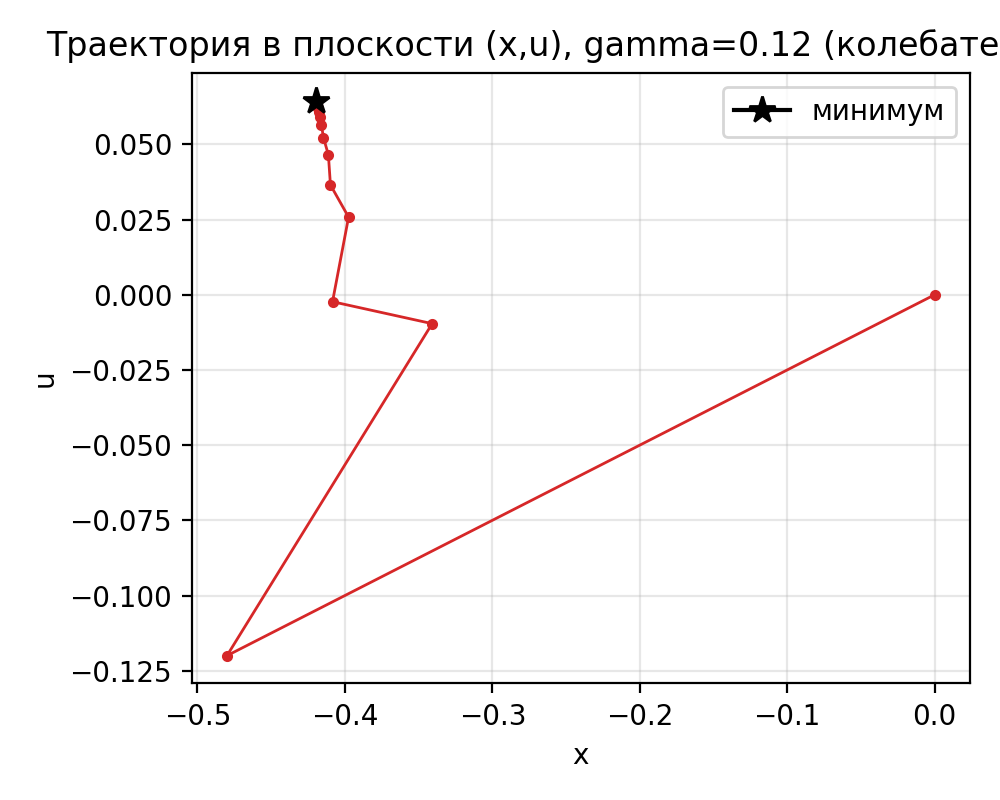
\includegraphics{task1/gd_traj_012.png}
        \caption{Траектория (x,u), $\gamma=0.12$}
    \end{subfigure}\hfill
    \begin{subfigure}{0.48\textwidth}
        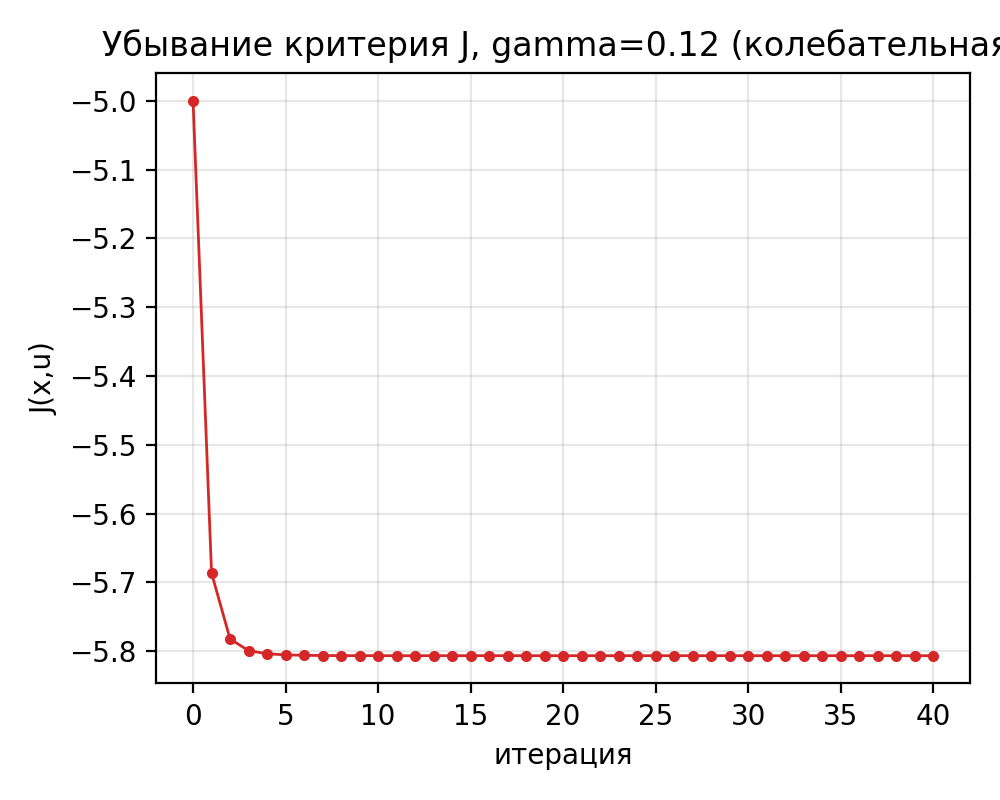
\includegraphics{task1/gd_J_012.png}
        \caption{$J$ по итерациям, $\gamma=0.12$}
    \end{subfigure}

    \vspace{0.5em}

    \begin{subfigure}{0.48\textwidth}
        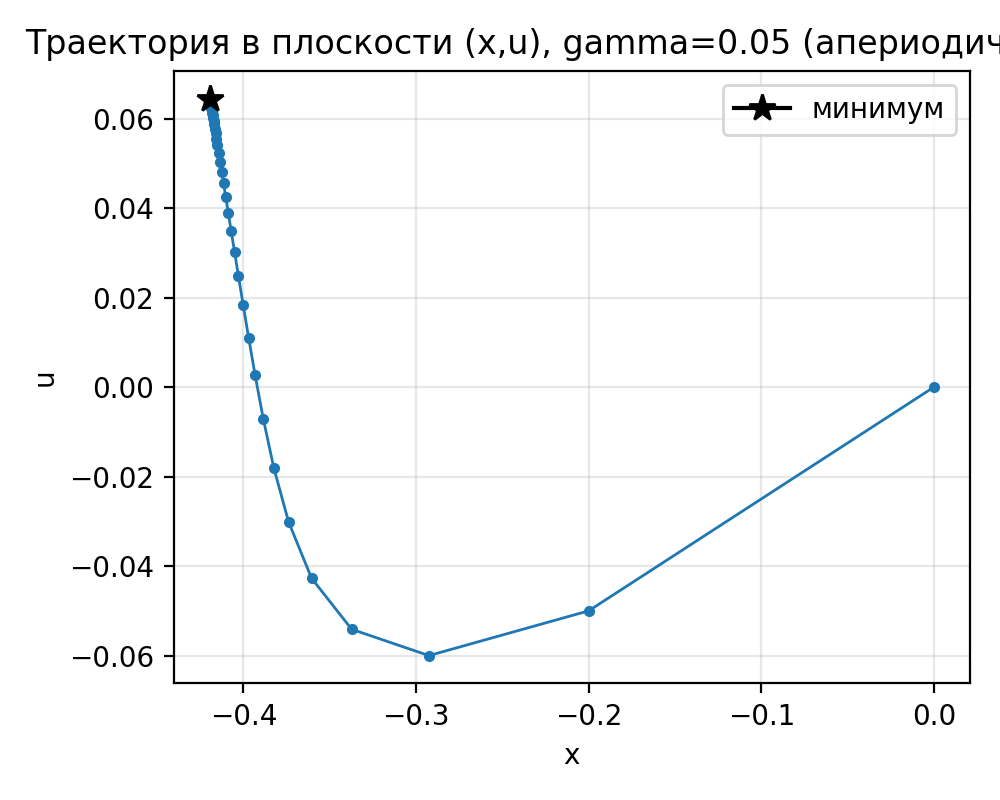
\includegraphics{task1/gd_traj_005.png}
        \caption{Траектория (x,u), $\gamma=0.05$}
    \end{subfigure}\hfill
    \begin{subfigure}{0.48\textwidth}
        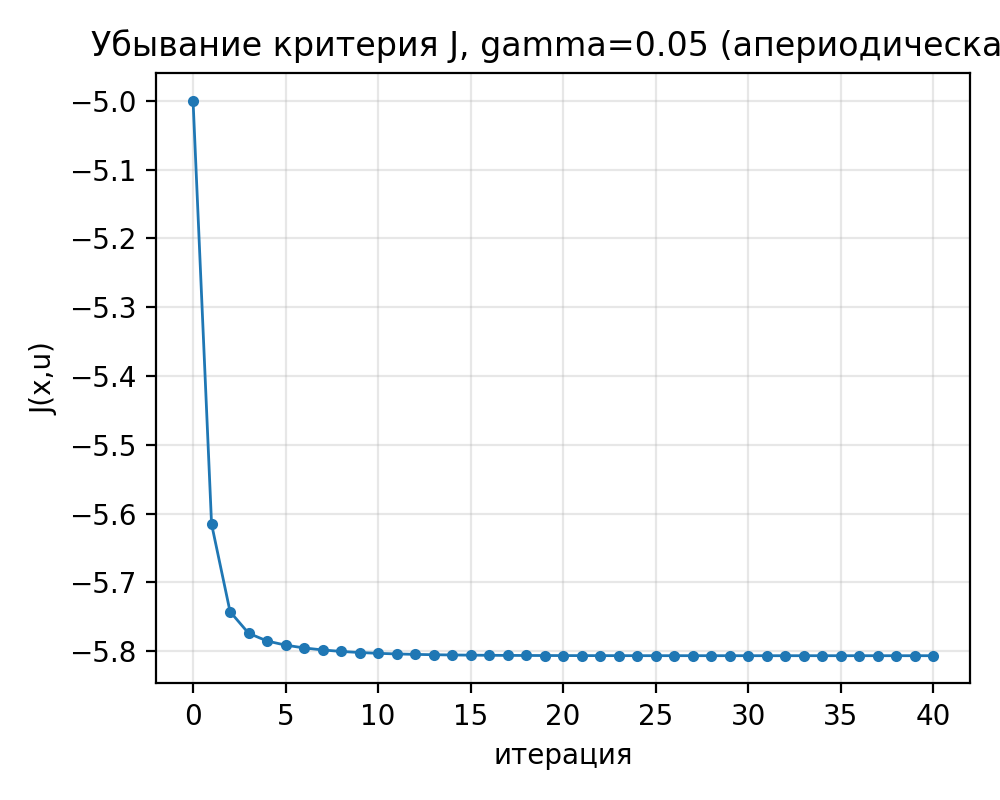
\includegraphics{task1/gd_J_005.png}
        \caption{$J$ по итерациям, $\gamma=0.05$}
    \end{subfigure}
    \caption{Градиентный спуск: сравнение траекторий и убывания $J$ для двух шагов}
    \label{fig:gd}
\end{figure}
